% Options for packages loaded elsewhere
\PassOptionsToPackage{unicode}{hyperref}
\PassOptionsToPackage{hyphens}{url}
%
\documentclass[
]{article}
\title{Equine Turnout at St.~Lawrence University}
\usepackage{etoolbox}
\makeatletter
\providecommand{\subtitle}[1]{% add subtitle to \maketitle
  \apptocmd{\@title}{\par {\large #1 \par}}{}{}
}
\makeatother
\subtitle{Clara Mugnai}
\author{}
\date{\vspace{-2.5em}}

\usepackage{amsmath,amssymb}
\usepackage{lmodern}
\usepackage{iftex}
\ifPDFTeX
  \usepackage[T1]{fontenc}
  \usepackage[utf8]{inputenc}
  \usepackage{textcomp} % provide euro and other symbols
\else % if luatex or xetex
  \usepackage{unicode-math}
  \defaultfontfeatures{Scale=MatchLowercase}
  \defaultfontfeatures[\rmfamily]{Ligatures=TeX,Scale=1}
\fi
% Use upquote if available, for straight quotes in verbatim environments
\IfFileExists{upquote.sty}{\usepackage{upquote}}{}
\IfFileExists{microtype.sty}{% use microtype if available
  \usepackage[]{microtype}
  \UseMicrotypeSet[protrusion]{basicmath} % disable protrusion for tt fonts
}{}
\makeatletter
\@ifundefined{KOMAClassName}{% if non-KOMA class
  \IfFileExists{parskip.sty}{%
    \usepackage{parskip}
  }{% else
    \setlength{\parindent}{0pt}
    \setlength{\parskip}{6pt plus 2pt minus 1pt}}
}{% if KOMA class
  \KOMAoptions{parskip=half}}
\makeatother
\usepackage{xcolor}
\IfFileExists{xurl.sty}{\usepackage{xurl}}{} % add URL line breaks if available
\IfFileExists{bookmark.sty}{\usepackage{bookmark}}{\usepackage{hyperref}}
\hypersetup{
  pdftitle={Equine Turnout at St.~Lawrence University},
  hidelinks,
  pdfcreator={LaTeX via pandoc}}
\urlstyle{same} % disable monospaced font for URLs
\usepackage[margin=1in]{geometry}
\usepackage{color}
\usepackage{fancyvrb}
\newcommand{\VerbBar}{|}
\newcommand{\VERB}{\Verb[commandchars=\\\{\}]}
\DefineVerbatimEnvironment{Highlighting}{Verbatim}{commandchars=\\\{\}}
% Add ',fontsize=\small' for more characters per line
\usepackage{framed}
\definecolor{shadecolor}{RGB}{248,248,248}
\newenvironment{Shaded}{\begin{snugshade}}{\end{snugshade}}
\newcommand{\AlertTok}[1]{\textcolor[rgb]{0.94,0.16,0.16}{#1}}
\newcommand{\AnnotationTok}[1]{\textcolor[rgb]{0.56,0.35,0.01}{\textbf{\textit{#1}}}}
\newcommand{\AttributeTok}[1]{\textcolor[rgb]{0.77,0.63,0.00}{#1}}
\newcommand{\BaseNTok}[1]{\textcolor[rgb]{0.00,0.00,0.81}{#1}}
\newcommand{\BuiltInTok}[1]{#1}
\newcommand{\CharTok}[1]{\textcolor[rgb]{0.31,0.60,0.02}{#1}}
\newcommand{\CommentTok}[1]{\textcolor[rgb]{0.56,0.35,0.01}{\textit{#1}}}
\newcommand{\CommentVarTok}[1]{\textcolor[rgb]{0.56,0.35,0.01}{\textbf{\textit{#1}}}}
\newcommand{\ConstantTok}[1]{\textcolor[rgb]{0.00,0.00,0.00}{#1}}
\newcommand{\ControlFlowTok}[1]{\textcolor[rgb]{0.13,0.29,0.53}{\textbf{#1}}}
\newcommand{\DataTypeTok}[1]{\textcolor[rgb]{0.13,0.29,0.53}{#1}}
\newcommand{\DecValTok}[1]{\textcolor[rgb]{0.00,0.00,0.81}{#1}}
\newcommand{\DocumentationTok}[1]{\textcolor[rgb]{0.56,0.35,0.01}{\textbf{\textit{#1}}}}
\newcommand{\ErrorTok}[1]{\textcolor[rgb]{0.64,0.00,0.00}{\textbf{#1}}}
\newcommand{\ExtensionTok}[1]{#1}
\newcommand{\FloatTok}[1]{\textcolor[rgb]{0.00,0.00,0.81}{#1}}
\newcommand{\FunctionTok}[1]{\textcolor[rgb]{0.00,0.00,0.00}{#1}}
\newcommand{\ImportTok}[1]{#1}
\newcommand{\InformationTok}[1]{\textcolor[rgb]{0.56,0.35,0.01}{\textbf{\textit{#1}}}}
\newcommand{\KeywordTok}[1]{\textcolor[rgb]{0.13,0.29,0.53}{\textbf{#1}}}
\newcommand{\NormalTok}[1]{#1}
\newcommand{\OperatorTok}[1]{\textcolor[rgb]{0.81,0.36,0.00}{\textbf{#1}}}
\newcommand{\OtherTok}[1]{\textcolor[rgb]{0.56,0.35,0.01}{#1}}
\newcommand{\PreprocessorTok}[1]{\textcolor[rgb]{0.56,0.35,0.01}{\textit{#1}}}
\newcommand{\RegionMarkerTok}[1]{#1}
\newcommand{\SpecialCharTok}[1]{\textcolor[rgb]{0.00,0.00,0.00}{#1}}
\newcommand{\SpecialStringTok}[1]{\textcolor[rgb]{0.31,0.60,0.02}{#1}}
\newcommand{\StringTok}[1]{\textcolor[rgb]{0.31,0.60,0.02}{#1}}
\newcommand{\VariableTok}[1]{\textcolor[rgb]{0.00,0.00,0.00}{#1}}
\newcommand{\VerbatimStringTok}[1]{\textcolor[rgb]{0.31,0.60,0.02}{#1}}
\newcommand{\WarningTok}[1]{\textcolor[rgb]{0.56,0.35,0.01}{\textbf{\textit{#1}}}}
\usepackage{graphicx}
\makeatletter
\def\maxwidth{\ifdim\Gin@nat@width>\linewidth\linewidth\else\Gin@nat@width\fi}
\def\maxheight{\ifdim\Gin@nat@height>\textheight\textheight\else\Gin@nat@height\fi}
\makeatother
% Scale images if necessary, so that they will not overflow the page
% margins by default, and it is still possible to overwrite the defaults
% using explicit options in \includegraphics[width, height, ...]{}
\setkeys{Gin}{width=\maxwidth,height=\maxheight,keepaspectratio}
% Set default figure placement to htbp
\makeatletter
\def\fps@figure{htbp}
\makeatother
\setlength{\emergencystretch}{3em} % prevent overfull lines
\providecommand{\tightlist}{%
  \setlength{\itemsep}{0pt}\setlength{\parskip}{0pt}}
\setcounter{secnumdepth}{-\maxdimen} % remove section numbering
\usepackage{booktabs}
\usepackage{longtable}
\usepackage{array}
\usepackage{multirow}
\usepackage{wrapfig}
\usepackage{float}
\usepackage{colortbl}
\usepackage{pdflscape}
\usepackage{tabu}
\usepackage{threeparttable}
\usepackage{threeparttablex}
\usepackage[normalem]{ulem}
\usepackage{makecell}
\usepackage{xcolor}
\ifLuaTeX
  \usepackage{selnolig}  % disable illegal ligatures
\fi

\begin{document}
\maketitle

\hypertarget{introduction}{%
\section{Introduction}\label{introduction}}

This project is an exploration of turnout preferences for horses both in
the St.~Lawrence University riding program and boarding at the school's
barn. Elsa Gunnison Appleton Riding Hall, in Canton, NY is the facility
where all of the horses were located and all of the data was gathered.
The horses were turned out in rotations based on where they had
previously done well outside. They were then observed and various
behaviors were recorded.

Some variables of interest in the study were:

\begin{itemize}
\tightlist
\item
  Time\_of\_day - the time of day when that observation was recorded
\item
  Age - the age of the particular horse being observed
\item
  Personality - based on the four major personalities of horses, this is
  the personality type of that particular horse
\item
  Date - the date which the observation was taken
\item
  Flymask - a 1 if the horse wore a fly mask that day, a 0 if they did
  not
\item
  Flysheet - a 1 if the horse wore a fly sheet that day, a 0 if they did
  not
\item
  Group - a 1 if the horse was in a group (2+), a 0 if they were not
\item
  Type\_of\_turnout - The name of the space the horse was turned out in
  (Image 1)
\item
  Frequency\_of\_trail\_swishes - how often the horse swished its tail
  in turnout (frequent, often, infrequent, or rare)
\item
  Minutes\_grazing - how many minutes of the 30 observed that the horse
  spent grazing
\item
  Dialated\_nostrils - how many times the horse exhibited dialated
  nostrils in turnout
\item
  Rigid\_body\_posture - how many times the horse exhibited a rigid,
  tense body posture
\item
  minutes\_spent\_pacing - how many minutes of the 30 observed that the
  horse spent pacing
\item
  number\_whinnies - how many times the horse whinnied in the 30 minutes
  observed
\item
  number\_positive\_interactions\_w/friends - refer to Methods
\item
  number\_negative\_interactions\_w/friends - refer to Methods
\item
  time\_layingdown - minutes spent of the 30 observed, with the horse
  laying down
\end{itemize}

There are four different personality types for horses and each type can
be grouped into either passive or aggressive (Barteau). Barteau is a
U.S. national champion dressage rider, and discusses the four types of
horse personalities that are seen in domestic horses. The types are
social, fearful, challenging, and aloof. She goes into detail with the
characteristics of each type and the ``1-10'' scale of those
personalities. She also states that there is a passive to aggressive
scale that applies to each type. Finally, the article goes into how to
determine a specific horse's type and which behaviors and reactions can
help to identify the type of personality that is being presented. This
was used as a model for how personalities of horses within this study
were determined.

An article by Foster also identifies horse personalities, the same four
types as Barteau. The main focus of Foster's article is the way horses
express discomfort with minimal movement. She identifies that the eyes
and other facial indicators are the most informative signals and that
changes in body posture and natural movement are other signals to how a
horse feels in turnout (2019). She also discusses that certain horses
have different baselines, and these behaviors are universally signals of
discomfort.

Foster's article was used heavily as a way to determine what should be
taken into account when observing horses. There were certain
accommodations made for the fact that there was a single researcher
doing all of the observations, specifically the times of day and the
scale for the number of tail swishes. The outside research completed by
others, as well as personal experience by the researcher, weighed into
the way the numerical scales were done. There was more emphasis on if a
horse was grazing or calmly moving around the space than on how many
times something alerted them. The overall way they behave in turnout
better indicates the contentedness of the horse than small moments of
spooking or alarm (Foster, Barteau).

\hypertarget{methods}{%
\section{Methods}\label{methods}}

Site Map: Elsa Gunnison Appleton Riding Hall

\begin{figure}
\centering
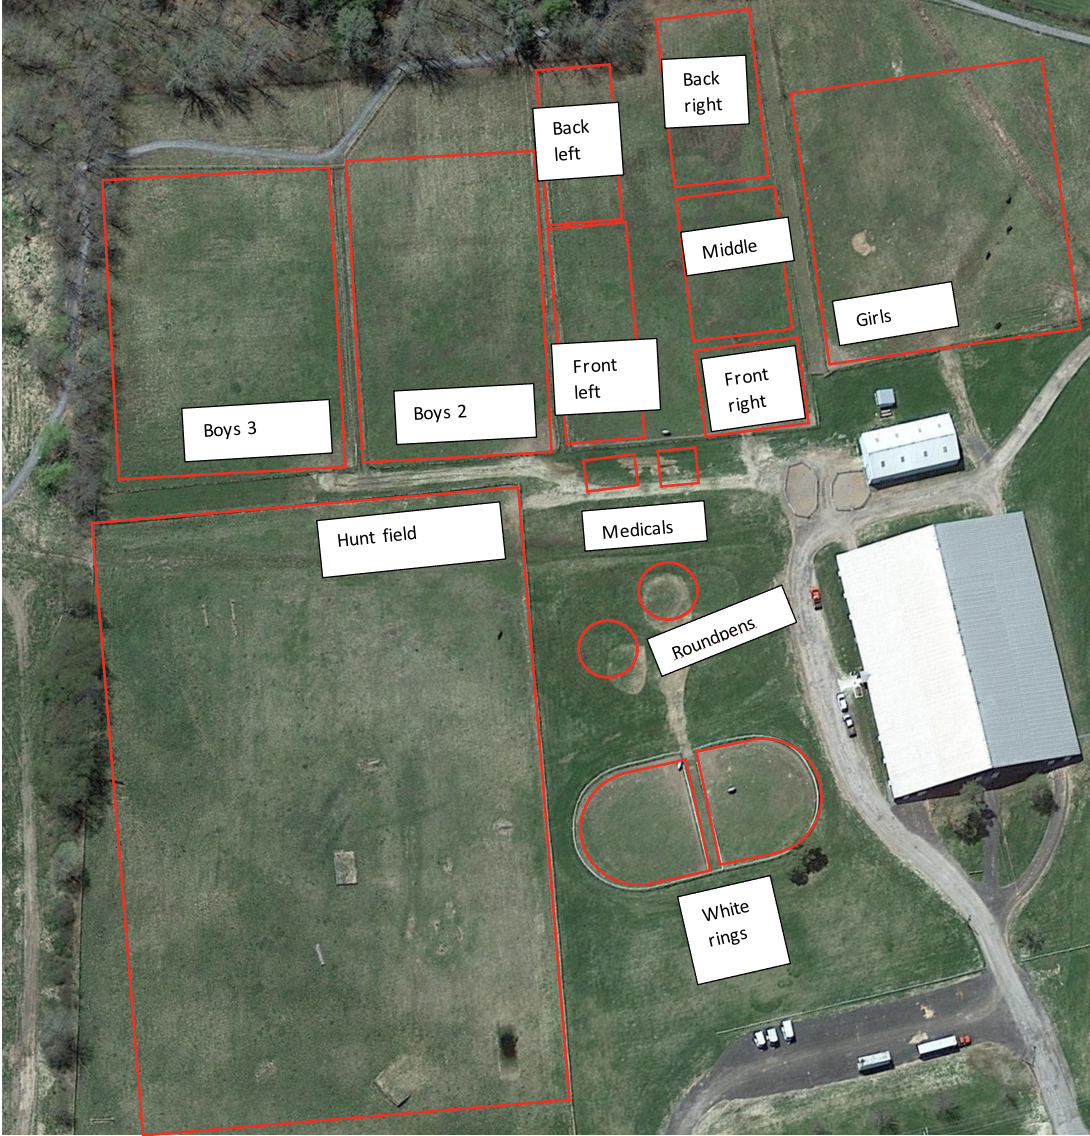
\includegraphics{/Users/claramugnai/Desktop/Spring 2022/SYE/SYE_spring2022/turnoutmap.png}
\caption{Image 1: layout of turnout spaces at St.~Lawrence Universities,
Elsa Gunnison Appleton Riding Hall}
\end{figure}

Horses were observed for 30-minute intervals in their natural turnout
environments and groups. The intervals in which they were observed were
randomized as much as possible, as well as the locations they were in.
My personal class schedule and the weather dictated which days and times
worked to observe in, and I attempted to rotate through the fields the
same way the entire time I took observations. I started in the white
rings and moved in a clockwise direction around the fields (white rings,
round-pens, medicals, hunt field, boys 3, boys 2,etc). The horses take
turns going out, at the discretion of the barn manager, and that is not
a set schedule so the ones being observed changed each week.

It is important to note that the turnout location of a medical has no
grass for them to graze on, only hay put there by humans, so those
observations are not well represented by grazing time. During
observation time it was noted how many minutes were spent both grazing
(a positive behavior) and pacing (a negative behavior), while
acknowledging that they could be doing neither of those things. In
addition to that, the number of times they whinnied, dilated their
nostrils, or had a rigid body posture were noted as negative signs in
turnout. For horses both alone and with friends in turnout it was noted
how many positive or negative social interactions they had with each
other. Positive interactions were things like nuzzling or grooming and
negative were running, chasing, or causing one another distress. Horses
in solitary turnout could still be bothered or settled down by
neighboring horses so they could have positive or negative interactions,
as well. Finally, it was noted how often the horses were swishing their
tails with the following scale, having both positive and negative
impacts:

\begin{itemize}
\tightlist
\item
  Frequent -- almost constant -- score 4 negative
\item
  Often -- regularly -- score 2 negative
\item
  Infrequent -- some but not overly obvious -- score 2 positive
\item
  Rare -- hardly ever -- score 4 positive
\end{itemize}

Note: The scale used for finding these numbers was arbitrary, and chosen
for the fact that it made sense given the importance of tail swishing
compared to the overall turnout scores for each horse. The total number
of tail swishes per horse, per observation session, were not possible to
be observed so this scale was chosen instead.

Upon the completion of data collection, overall turnout scores were
calculated. This was done by adding the minutes grazing, tail swishing
score (if positive), positive friend interactions, and minutes laying
down together to be a positive score. Negative scores were; the sum of
minutes pacing, tail swishing score (if negative), occurrences of body
tension, whinnying, nostril dilation, and negative friend interactions
(Foster). Choosing to add these numbers together was a subjective
decision because every observation was 30 minutes long and all of the
things that indicated a pleasant time for the horse were considered
positive, all of the unpleasant things were considered negative (Paddock
Anxiety). The positive and negative scores were then added together to
give an overall turnout score.

For any horses that appeared 3 or more times in the data set, their
observations were included in the final data set. Those horses were each
then observed for approximately 10 minutes in the barn to quickly assess
their personality types. In those 10 minutes they were exposed to new
stimuli in the form of a human, another horse, and a foreign object to
see how they reacted. Based on those reactions they were classified as
either social, aloof, challenging, or fearful. For each type there was
both a passive or aggressive form, depending on how fast or intense the
reactions to the stimuli were (Barteau).

\hypertarget{exploratory-analysis}{%
\section{Exploratory Analysis}\label{exploratory-analysis}}

\begin{Shaded}
\begin{Highlighting}[]
\FunctionTok{library}\NormalTok{(tidyverse)}
\FunctionTok{library}\NormalTok{(ggplot2)}
\FunctionTok{library}\NormalTok{(readxl)}
\FunctionTok{library}\NormalTok{(dplyr)}
\FunctionTok{library}\NormalTok{(lme4)}
\FunctionTok{library}\NormalTok{(knitr)}
\FunctionTok{library}\NormalTok{(pander)}
\FunctionTok{library}\NormalTok{(ggthemes)}
\FunctionTok{library}\NormalTok{(kableExtra)}
\FunctionTok{library}\NormalTok{(rmdformats)}
\FunctionTok{library}\NormalTok{(hms)}
\NormalTok{turnout\_data }\OtherTok{\textless{}{-}} \FunctionTok{read\_excel}\NormalTok{(}\StringTok{"SYE data sheet.xlsx"}\NormalTok{,}
 \AttributeTok{col\_types =} \FunctionTok{c}\NormalTok{(}
\NormalTok{ ))}

\NormalTok{turnout\_data }\OtherTok{\textless{}{-}}\NormalTok{ turnout\_data }\SpecialCharTok{\%\textgreater{}\%} \FunctionTok{mutate}\NormalTok{(}\AttributeTok{Flymask =} \FunctionTok{if\_else}\NormalTok{(Flymask }\SpecialCharTok{==} \StringTok{"x"}\NormalTok{, }\StringTok{"Yes"}\NormalTok{,}\StringTok{"No"}\NormalTok{)) }\SpecialCharTok{\%\textgreater{}\%} 
  \FunctionTok{mutate}\NormalTok{(}\AttributeTok{Flysheet =} \FunctionTok{if\_else}\NormalTok{(Flysheet }\SpecialCharTok{==} \StringTok{"x"}\NormalTok{, }\StringTok{"Yes"}\NormalTok{, }\StringTok{"No"}\NormalTok{)) }\SpecialCharTok{\%\textgreater{}\%}
  \FunctionTok{mutate}\NormalTok{(}\AttributeTok{Group =} \FunctionTok{if\_else}\NormalTok{(Group }\SpecialCharTok{==} \StringTok{"x"}\NormalTok{, }\StringTok{"Yes"}\NormalTok{, }\StringTok{"No"}\NormalTok{)) }\SpecialCharTok{\%\textgreater{}\%}
  \FunctionTok{replace}\NormalTok{(}\FunctionTok{is.na}\NormalTok{(.), }\StringTok{"No"}\NormalTok{) }\SpecialCharTok{\%\textgreater{}\%}  
  \FunctionTok{mutate}\NormalTok{(}\AttributeTok{Horse =} \FunctionTok{fct\_reorder}\NormalTok{(Horse, Totalnegativesigns)) }\SpecialCharTok{\%\textgreater{}\%}
 \FunctionTok{arrange}\NormalTok{(Totalnegativesigns) }
\end{Highlighting}
\end{Shaded}

\hypertarget{tables}{%
\subsubsection{Tables}\label{tables}}

The variable of ``Total Negative Signs'' will be used instead of
``overall'' turnout score because it has less bias towards horses in
turnout areas with grass.

\begin{table}

\caption{\label{tab:unnamed-chunk-2}Average Number of Negative Signs for each Horse}
\fontsize{20}{22}\selectfont
\begin{tabular}[t]{l|r}
\hline
Horse & Average Negative Signs\\
\hline
\textcolor{olivedrab3}{Cortez} & \textcolor{olivedrab3}{0.00}\\
\hline
Lucy & 0.00\\
\hline
Bling & 0.33\\
\hline
Cenvia & 0.33\\
\hline
Cheeto & 2.67\\
\hline
Juno & 3.00\\
\hline
Tucker & 3.00\\
\hline
Oscar & 5.00\\
\hline
Kirk & 5.00\\
\hline
Monroe & 5.00\\
\hline
Mouse & 5.40\\
\hline
Vox & 5.75\\
\hline
Epsom & 7.00\\
\hline
Obi & 9.33\\
\hline
Patches & 14.00\\
\hline
Milo & 17.00\\
\hline
Logan & 17.00\\
\hline
Henry & 21.00\\
\hline
\end{tabular}
\end{table}

\begin{table}

\caption{\label{tab:unnamed-chunk-3}Average Number of Negative Signs for each Personality}
\centering
\begin{tabular}[t]{l|r|r}
\hline
Personality & Average Negative Signs & Sample Size\\
\hline
Challenging - Passive & 2.67 & 3\\
\hline
Aloof - Passive & 3.12 & 17\\
\hline
Social - Passive & 3.36 & 11\\
\hline
Aloof - Aggressive & 5.00 & 3\\
\hline
Challenging - Aggressive & 5.75 & 4\\
\hline
Social - Aggressive & 8.60 & 15\\
\hline
Fearful - Passive & 19.00 & 6\\
\hline
\end{tabular}
\end{table}

\hypertarget{boxplots}{%
\subsubsection{Boxplots}\label{boxplots}}

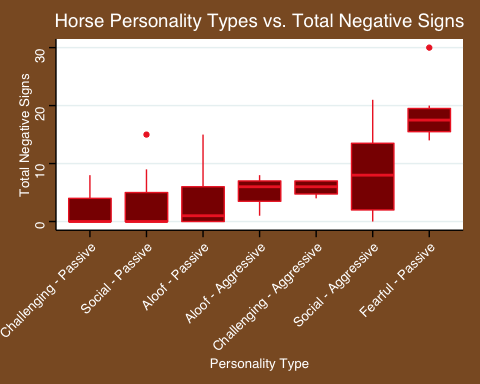
\includegraphics{Final_writeup_files/figure-latex/unnamed-chunk-4-1.pdf}

Interesting things happening here but the small number of observations
per group must be noted.

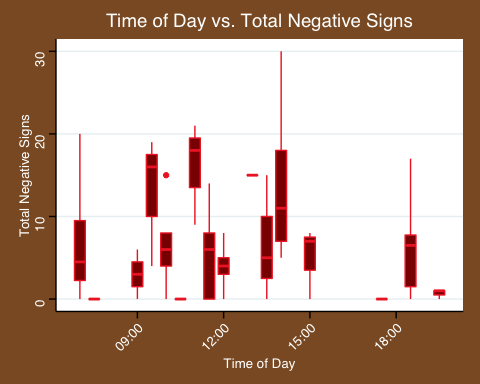
\includegraphics{Final_writeup_files/figure-latex/unnamed-chunk-5-1.pdf}

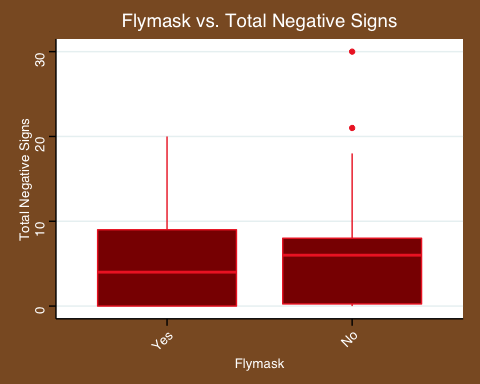
\includegraphics{Final_writeup_files/figure-latex/unnamed-chunk-6-1.pdf}

This is showing a difference with the biggest takeaway from this plot
being that there are two outliers in the ``no flymask'' category.

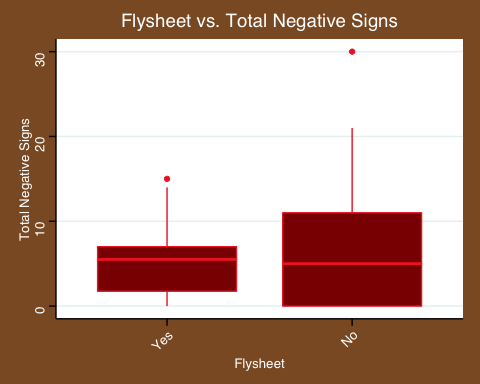
\includegraphics{Final_writeup_files/figure-latex/unnamed-chunk-7-1.pdf}

There is not a large difference here, with very similar medians for each
group. Again, the outliers are the most significant things in this plot.
It can be noted that there is more variation in the no flymask category
than in the flymask category.

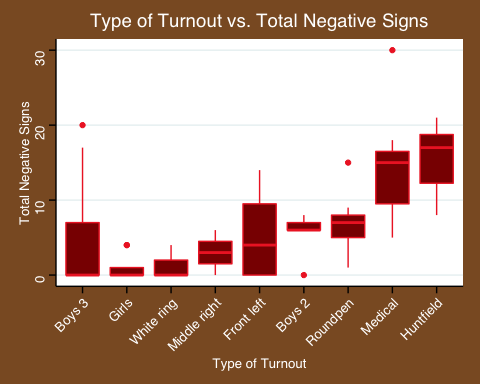
\includegraphics{Final_writeup_files/figure-latex/unnamed-chunk-8-1.pdf}

It looks like certain fields have more success but it also needs to be
considered which horses go in those fields. For example, the medical
paddocks and the roundpens are the closest in proximity to the barn and
hold the least relaxed horses. Those fields also have two of the highest
negative scores. However, if horses were randomly assigned to fields
that would probably not be the case.

\hypertarget{scatterplots}{%
\subsubsection{Scatterplots}\label{scatterplots}}

In this section, each point is representing a single observation period.
So there are 3-4 points per horse, and 59 points total on each graph.

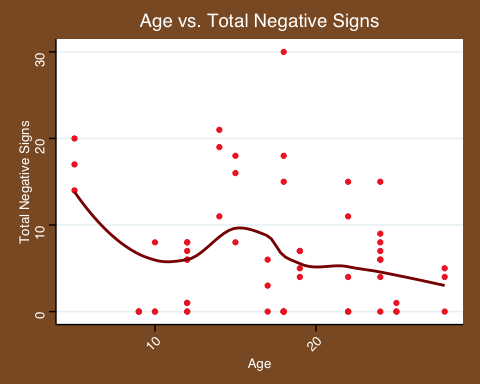
\includegraphics{Final_writeup_files/figure-latex/unnamed-chunk-9-1.pdf}
There does not seem to be a strong relationship between age and the
number of negative signs. The slight downward trend may be due to the
small sample sizes at the ends of the trend line, in the center where
there are more data points there is less of a trend.

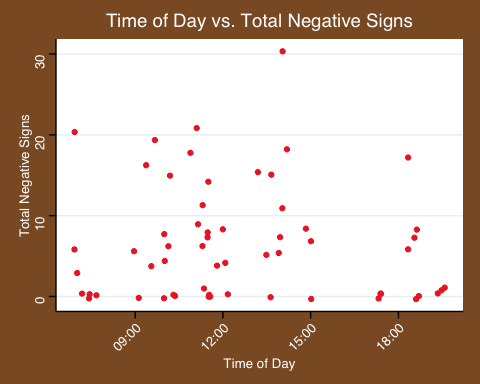
\includegraphics{Final_writeup_files/figure-latex/unnamed-chunk-10-1.pdf}
There appears to be no trend in total negative signs as the time of day
for turnout changes.

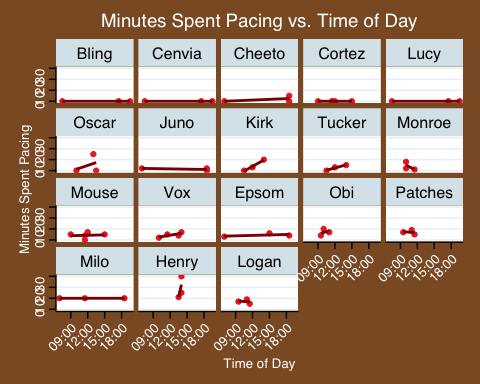
\includegraphics{Final_writeup_files/figure-latex/unnamed-chunk-11-1.pdf}
There are a lot of different slopes showing here for the different
horses, mainly due to the fact that there are only three observations
per horse.

\hypertarget{comparing-different-slopes-in-scatterplots}{%
\subsubsection{Comparing different Slopes in
Scatterplots}\label{comparing-different-slopes-in-scatterplots}}

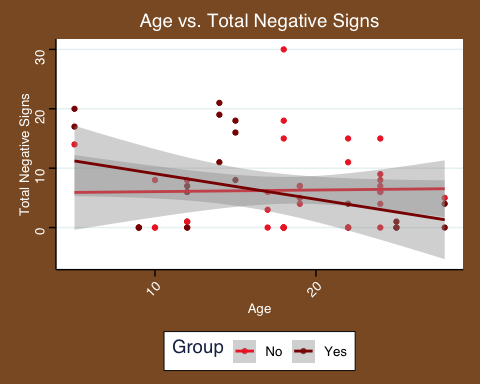
\includegraphics{Final_writeup_files/figure-latex/unnamed-chunk-12-1.pdf}

Exploring multilevel scenarios, it looks like Age and Group may be
related, with different slopes for group and non-group, so as age
increases in a group the group does better but as age increases in
individual horses they do worse.

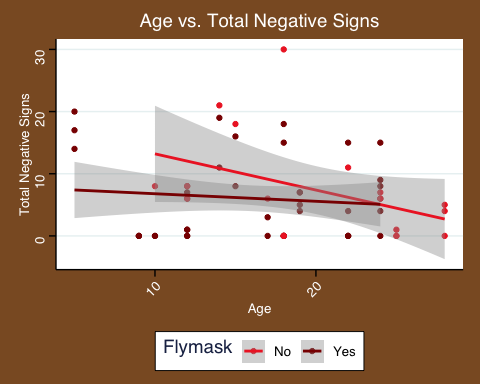
\includegraphics{Final_writeup_files/figure-latex/unnamed-chunk-13-1.pdf}

Flymask also seems to have significant differences in slopes and
intercepts.

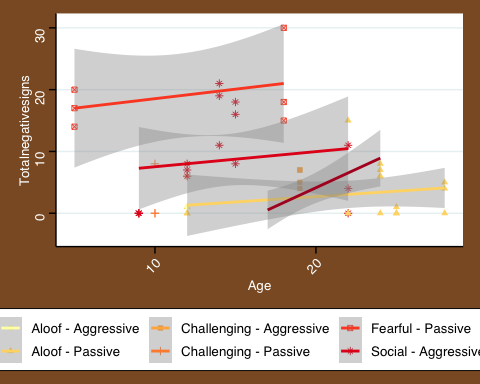
\includegraphics{Final_writeup_files/figure-latex/unnamed-chunk-14-1.pdf}

\begin{verbatim}
## $y
## [1] "Total Negative Signs"
## 
## $x
## [1] "Age"
## 
## $title
## [1] "Age vs. Total Negative Signs"
## 
## attr(,"class")
## [1] "labels"
\end{verbatim}

The different personalities definitely are different, and we have seen
that each horse is different so we do need to account for the grouped
horses. the personalities seem to make a difference in the slopes here
but we have to be mindful of the fact that there are very few of each
personalities.

\hypertarget{multilevel-unconditional-means-model}{%
\subsubsection{Multilevel Unconditional Means
Model}\label{multilevel-unconditional-means-model}}

Unconditional means model:

~

Totalnegativesigns

Predictors

Estimates

CI

p

(Intercept)

6.69

3.66~--~9.71

\textless0.001

Random Effects

σ2

16.58

τ00 Horse

35.79

ICC

0.68

N Horse

18

Observations

59

Marginal R2 / Conditional R2

0.000 / 0.683

Looking at the unconditional means model, the ICC value is 0.683, with a
significant p-value, so this is a multilevel data set and needs to be
allowed to have different intercepts for different horses.

\hypertarget{conclusion}{%
\subsubsection{Conclusion}\label{conclusion}}

Some take-aways from this are that personality type does seem to make
difference to horse success in turnout. Flymask use also seems to make a
difference to success in turnout. For interactions, it seems like age
and group seem to interact with turnout success, as well as ago and
flymask.

Limitations to this study are both few observations and a lack of
randomization. The modeling would be a lot more significant if there
were enough observations to result in significant and meaningful
p-values, and if randomization had been more attainable the issues with
field type causing a trend would not happen. Those things would make
this study a lot more applicable to be used beyond a singular viewing
tool, and instead as a predicting model.

\hypertarget{shiny-application}{%
\section{Shiny Application}\label{shiny-application}}

\hypertarget{citations}{%
\section{Citations}\label{citations}}

Barteau, Y. (2009, March 5). Understanding horse personalities, part 1:
The 4 basic personality types. Dressage Today. Retrieved December 9,
2021, from
\url{https://dressagetoday.com/theory/horse-personalities-basic-types}.

Chaya, L., Cowan, E., \& McGuire, B. (2006). A note on the relationship
between time spent in turnout and behavior during turnout in horses
(Equus caballus). Applied Animal Behavior Science, 98(1-2), 155--160.
\url{https://doi.org/10.1016/j.applanim.2005.08.020}

Foster, R. (2019, October 1). Recognizing pain in stoic horses. The
Horse. Retrieved December 9, 2021, from
\url{https://thehorse.com/113343/recognizing-pain-in-stoic-horses/}.

Paddock anxiety: How to help your horse relax. TRTmethod. (2020, October
12). Retrieved December 9, 2021, from
\url{https://www.trtmethod.com/separation-anxiety/how-to-deal-}
with-paddock-anxiety/.

\end{document}
